\documentclass{article}
\usepackage{tikz}
\usetikzlibrary{matrix, calc, positioning, arrows}
\usepackage{fontspec}
\setmainfont{[EncodeSans-Regular.ttf]}
\newfontfamily{\bold}{EncodeSans-Bold.ttf}

\begin{document}

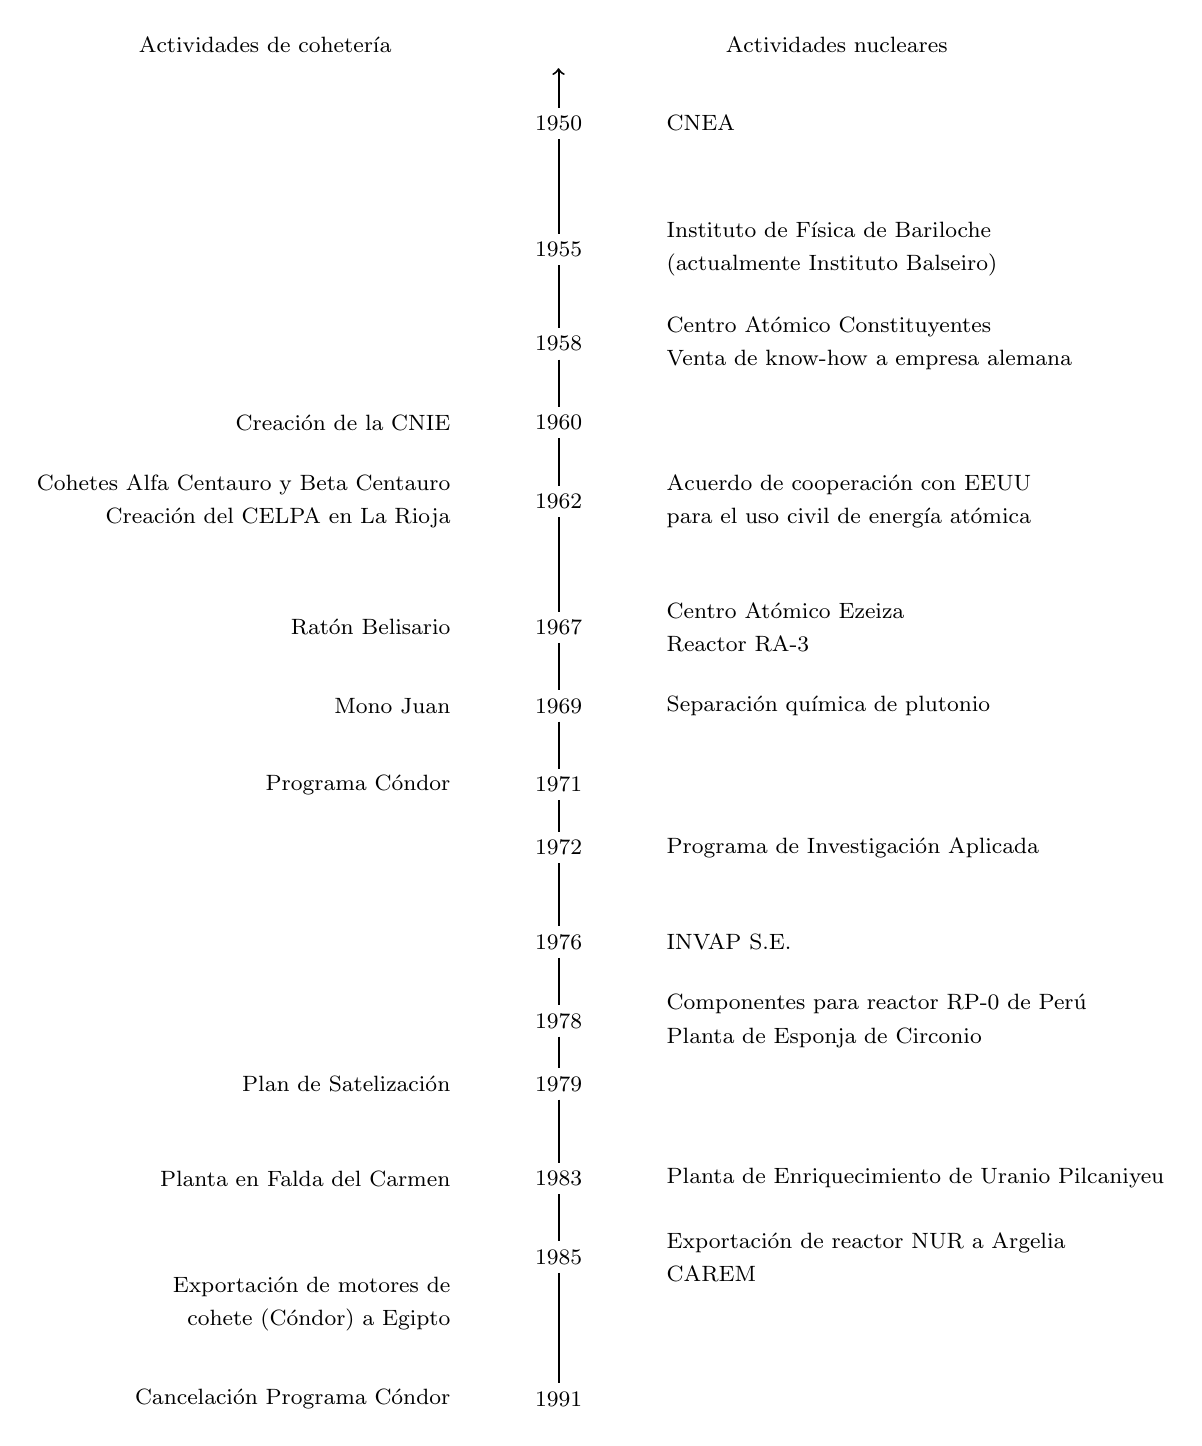
\begin{tikzpicture}

% Draw the timeline
\draw[line width=0.25mm, <-] (0,19.7) -- (0,19.2);
\draw[line width=0.25mm, -] (0,18.8) -- (0,17.6);
\draw[line width=0.25mm, -] (0,17.2) -- (0,16.4);
\draw[line width=0.25mm, -] (0,16) -- (0,15.4);
\draw[line width=0.25mm, -] (0,15) -- (0,14.4);
\draw[line width=0.25mm, -] (0,14) -- (0,12.8);
\draw[line width=0.25mm, -] (0,12.4) -- (0,11.8);
\draw[line width=0.25mm, -] (0,11.4) -- (0,10.8);
\draw[line width=0.25mm, -] (0,10.4) -- (0,10);
\draw[line width=0.25mm, -] (0,9.6) -- (0,8.8);
\draw[line width=0.25mm, -] (0,8.4) -- (0,7.8);
\draw[line width=0.25mm, -] (0,7.4) -- (0,7);
\draw[line width=0.25mm, -] (0,6.6) -- (0,5.8);
\draw[line width=0.25mm, -] (0,5.4) -- (0,4.8);
\draw[line width=0.25mm, -] (0,4.4) -- (0,3);

% Titles
\node [left, text centered] at (-2, 20) {\footnotesize \bold{Actividades de cohetería}};
\node [right, text centered] at (2, 20) {\footnotesize  \bold{Actividades nucleares}};

% Add the years as labels
\node at (0, 19) {\footnotesize \bold{1950}};
\node [right] at (1.25, 19) {\footnotesize CNEA};

\node at (0, 17.4) {\footnotesize \bold{1955}};
\node [right, align = left] at (1.25, 17.4) {\footnotesize Instituto de Física de Bariloche \\ \footnotesize (actualmente Instituto Balseiro)};

\node at (0, 16.2) {\footnotesize \bold{1958}};
\node [right, align = left] at (1.25, 16.2) {\footnotesize Centro Atómico Constituyentes \\ \footnotesize Venta de know-how a empresa alemana};

\node at (0, 15.2) {\footnotesize \bold{1960}};
\node [left] at (-1.25, 15.2) {\footnotesize Creación de la CNIE};

\node at (0, 14.2) {\footnotesize \bold{1962}};
\node [left, align = right] at (-1.25, 14.2) {\footnotesize Cohetes Alfa Centauro y Beta Centauro \\ \footnotesize Creación del CELPA en La Rioja};
\node [right, align = left] at (1.25, 14.2) {\footnotesize Acuerdo de cooperación con EEUU \\ \footnotesize para el uso civil de energía atómica};

\node at (0, 12.6) {\footnotesize \bold{1967}};
\node [left, align = right] at (-1.25, 12.6) {\footnotesize Ratón Belisario};
\node [right, align = left] at (1.25, 12.6) {\footnotesize Centro Atómico Ezeiza \\ \footnotesize Reactor RA-3};

\node at (0, 11.6) {\footnotesize \bold{1969}};
\node [right] at (1.25, 11.6) {\footnotesize Separación química de plutonio};
\node [left] at (-1.25, 11.6) {\footnotesize Mono Juan};

\node at (0, 10.6) {\footnotesize \bold{1971}};
\node [left] at (-1.25, 10.6) {\footnotesize Programa Cóndor};

\node at (0, 9.8) {\footnotesize \bold{1972}};
\node [right] at (1.25, 9.8) {\footnotesize Programa de Investigación Aplicada};

\node at (0, 8.6) {\footnotesize \bold{1976}};
\node [right] at (1.25, 8.6) {\footnotesize INVAP S.E.};

\node at (0, 7.6) {\footnotesize \bold{1978}};
\node [right, align = left] at (1.25, 7.6) {\footnotesize Componentes para reactor RP-0 de Perú \\ \footnotesize Planta de Esponja de Circonio};

\node at (0, 6.8) {\footnotesize \bold{1979}};
\node [left] at (-1.25, 6.8) {\footnotesize Plan de Satelización};

\node at (0, 5.6) {\footnotesize \bold{1983}};
\node [left] at (-1.25, 5.6) {\footnotesize Planta en Falda del Carmen};
\node [right] at (1.25, 5.6) {\footnotesize Planta de Enriquecimiento de Uranio Pilcaniyeu};

\node at (0, 4.6) {\footnotesize \bold{1985}};
\node [right, align = left] at (1.25, 4.6) {\footnotesize Exportación de reactor NUR a Argelia \\ \footnotesize CAREM};
\node [left, align = right] at (-1.25, 4) {\footnotesize Exportación de motores de \\ \footnotesize cohete (Cóndor) a Egipto};

\node at (0, 2.8) {\footnotesize \bold{1991}};
\node [left] at (-1.25, 2.8) {\footnotesize Cancelación Programa Cóndor};

\end{tikzpicture}

\end{document}